\chapter{Differentiation}
\section{Definition}
\prototype{$x^3$ has derivative $3x^2$.}

I suspect most of you have seen this before, but:
\begin{definition}
	Let $U$ be an open subset\footnote{We
		will almost always use $U = (a,b)$ or $U = \RR$,
		and you will not lose much by restricting
		the definition to those.}
	of $\RR$ and let $f \colon U \to \RR$ be a function.
	Let $p \in U$.
	We say $f$ is \vocab{differentiable} at $p$
	if the limit\footnote{Remember we are following the convention in
		\Cref{abuse:limit}.
		So we mean ``the limit of the function $h \mapsto \frac{f(p+h)-f(p)}{h}$
		except the value at $h=0$ can be anything''.
		And this is important because that fraction
		does not have a definition at $h = 0$.
		As promised, we pay this no attention.}
	\[ \lim_{h \to 0} \frac{f(p+h) - f(p)}{h} \]
	exists.
	If so, we denote its value by $f'(p)$ and refer
	to this as the \vocab{derivative} of $f$ at $p$.

	The function $f$ is differentiable if it is differentiable
	at every point.
	In that case, we regard the derivative $f' \colon (a,b) \to \RR$
	as a function it its own right.
\end{definition}

\begin{exercise}
	Show that if $f$ is differentiable at $p$
	then it is continuous at $p$ too.
\end{exercise}

Here is the picture.
Suppose $f \colon \RR \to \RR$ is differentiable
(hence continuous).
We draw a graph of $f$ in the usual way and consider values of $h$.
For any nonzero $h$, what we get is the slope of the \emph{secant}
line joining $(p, f(p))$ to $(p+h, f(p+h))$.
However, as $h$ gets close to zero,
that secant line begins to approach a line
which is tangent to the graph of the curve.
A picture with $f$ a parabola is shown below,
with the tangent in red, and the secant in dashed green.

\begin{center}
\begin{asy}
	import graph;
	size(8cm);
	real f(real x) { return (x-2)*(x-2)/2 - 0.1; }
	graph.xaxis("$x$");
	graph.yaxis("$y$");
	draw(graph(f,-1,5,operator ..), blue, Arrows);
	pair P = (3, f(3));
	dot("$(p, f(p))$", P, dir(-20), red);
	draw((1.8,-0.8)--(4.2, 1.6), red);
	label("Slope $f'(p)$", (4.2, 1.6), dir(-25), red);
	pair Q = (4.3, f(4.3));
	dot("$(p+h, f(p+h))$", Q, dir(-20), deepgreen);
	draw(P--Q, dashed+deepgreen);
	label("Slope $\frac{f(p+h)-f(p)}{h}$", P--Q, 1.5*dir(165), deepgreen);
\end{asy}
\end{center}

So the picture in your head should be that
\begin{moral}
	$f'(p)$ looks like the slope of the tangent line at $(p, f(p))$.
\end{moral}

\begin{remark}
	Note that the derivatives are defined
	for functions on \emph{open} intervals.
	This is important.
	If $f \colon [a,b] \to \RR$ for example,
	we could still define the derivative at each interior point,
	but $f(a)$ no longer makes sense
	since $f$ is not given a value on any open neighborhood of $a$.
\end{remark}

Let's do one computation and get on with this.
\begin{example}
	[Derivative of $x^3$ is $3x^2$]
	Let $f \colon \RR \to \RR$ by $f(x) = x^3$.
	For any point $p$, and \emph{nonzero} $h$ we can compute
	\begin{align*}
		\frac{f(p+h) - f(p)}{h} &= \frac{(p+h)^3 - p^3}{h} \\
		&= \frac{3p^2h + 3ph^2 + h^3}{h} \\
		&= 3p^2 + 3ph + h^2.
	\end{align*}
	Thus,
	\[ \lim_{h \to 0} \frac{f(p+h)-f(p)}{h}
		= \lim_{h \to 0} (3p^2+3ph+h^2) = 3p^2. \]
	Thus the slope at each point of $f$ is given by the formula $3p^2$.
	It is customary to then write $f'(x) = 3x^2$
	as the derivative of the entire function $f$.
\end{example}
\begin{abuse}
	We will now be sloppy and write this as $(x^3)' = 3x^2$.
	This is shorthand for the significantly more verbose
	``the real-valued function $x^3$ on domain so-and-so
	has derivative $3p^2$ at every point $p$ in its domain''.

	In general, a real-valued differentiable function
	$f \colon U \to \RR$ naturally gives rise to derivative
	$f'(p)$ at every point $p \in U$,
	so it is customary to just give up on $p$ altogether
	and treat $f'$ as function itself $U \to \RR$,
	even though this real number is of a ``different interpretation'':
	$f'(p)$ is meant to interpret a slope (e.g.\ your hourly pay rate)
	as opposed to a value (e.g.\ your total dollar worth at time $t$).
	If $f$ is a function from real life, the units do not even match!

	This convention is so deeply entrenched I cannot uproot it
	without more confusion than it is worth.
	But if you read the chapters on multivariable calculus
	you will see how it comes back to bite us,
	when I need to re-define the derivative to be a \emph{linear map},
	rather than single real numbers.
\end{abuse}

\section{How to compute them}
Same old, right?
Sum rule, all that jazz.

\begin{theorem}
	[Your friendly high school calculus rules]
	In what follows $f$ and $g$ are differentiable functions,
	and $U$, $V$ are open subsets of $\RR$.
	\begin{itemize}
		\ii (Sum rule) If $f,g \colon U \to \RR$ then
		then $(f+g)'(x) = f'(x) + g'(x)$.

		\ii (Product rule) If $f,g \colon U \to \RR$ then
		then $(f \cdot g)'(x) = f'(x) g(x) + f(x) g'(x)$.

		\ii (Chain rule) If $f \colon U \to V$ and $g \colon V \to \RR$
		then the derivative of the composed function
		$g \circ f \colon U \to \RR$ is $g'(f(x)) \cdot f'(x)$.
	\end{itemize}
\end{theorem}
\begin{proof}
	\begin{itemize}
	\ii Sum rule: trivial, do it yourself if you care.

	\ii Product rule: for every nonzero $h$ and point $p \in U$
	we may write
	\[
		\frac{f(p+h) g(p+h) - f(p) g(p)}{h}
		= \frac{f(p+h) - f(p)}{h} \cdot g(p+h)
		+ \frac{g(p+h)-g(p)}{h} \cdot f(p)
	\]
	which as $h \to 0$ gives the desired expression.

	\ii Chain rule: this is where \Cref{abuse:limit}
	will actually bite us.
	Let $p \in U$, $q = f(p) \in V$, so that
	\[ (g \circ f)'(p) = \lim_{h \to 0} \frac{g(f(p+h)) - g(q)}{h}. \]
	We would like to write the expression in the limit as
	\[ \frac{g(f(p+h)) - g(q)}{h}
		= \frac{g(f(p+h)) - g(q)}{f(p+h) - q}
		\cdot \frac{f(p+h) - f(p)}{h}. \]
	The problem is that the denominator $f(p+h)-f(p)$ might be zero.
	So instead, we define the expression
	\[
		Q(y) = \begin{cases}
			\frac{g(y) - g(q)}{y - q} & \text{if } y \ne q \\
			g'(q) & \text{if } y = q
		\end{cases}
	\]
	which is continuous since $g$ was differentiable at $q$.
	Then, we \emph{do} have the equality
	\[ \frac{g(f(p+h)) - g(q)}{h}
		= Q\left( f(p+h) \right) \cdot \frac{f(p+h) - f(p)}{h}. \]
	because if $f(p+h) = q$ with $h \ne 0$,
	then both sides are equal to zero anyways.

	Then, in the limit as $h \to 0$,
	we have $\lim_{h \to 0} \frac{f(p+h)-f(p)}{h} = f'(p)$,
	while $\lim_{h \to 0} Q(f(p+h)) = Q(q) = g'(q)$ by continuity.
	This was the desired result. \qedhere
	\end{itemize}
\end{proof}

\begin{exercise}
	Compute the derivative of the polynomial $f(x) = x^3 + 10x^2 + 2019$,
	viewed as a function $f \colon \RR \to \RR$.
\end{exercise}

\begin{remark}
	Quick linguistic point:
	the theorems above all hold at each individual point.
	For example the sum rule really should say that
	if $f,g \colon U \to \RR$ are differentiable at the point $p$
	then so is $f+g$ and the derivative equals $f'(p) + g'(p)$.
	Thus $f$ and $g$ are differentiable on all of $U$,
	then it of course follows that $(f+g)' = f' + g'$.
	So each of the above rules has a ``point-by-point'' form
	which then implies the ``whole $U$'' form.

	We only state the latter since that is what is used in practice.
	However, in the rare situations where you have a function
	differentiable only at certain points of $U$ rather
	than the whole interval $U$, you can still use the below.
\end{remark}

We next list some derivatives of
well-known functions,
but as we do not give rigorous definitions
of these functions, we do not prove these here.
\begin{proposition}
	[Derivatives of some well-known functions]
	\listhack
	\begin{itemize}
		\ii The exponential function $\exp \colon \RR \to \RR$
		defined by $\exp(x) = e^x$ is its own derivative.
		\ii The trig functions $\sin$ and $\cos$
		have $\sin' = \cos$, $\cos' = -\sin$.
	\end{itemize}
\end{proposition}

\begin{example}
	[A typical high-school calculus question]
	This means that you can mechanically compute
	the derivatives of any artificial function obtained by using the above,
	which makes it a great source of busy work
	in American high schools and universities.
	For example, if
	\[ f(x) = e^x + x \sin(x^2) \qquad f \colon \RR \to \RR \]
	then one can compute $f'$ by:
	\begin{align*}
		f'(x) &= (e^x)' + (x \sin(x^2))' & \text{sum rule} \\
		&= e^x + (x \sin(x^2))' & \text{above table} \\
		&= e^x + (x)' \sin(x^2) + x (\sin(x^2))' & \text{product rule} \\
		&= e^x + \sin(x^2) + x (\sin(x^2))' & (x)' = 1 \\
		&= e^x + \sin(x^2) + x \cdot 2x \cdot \cos(x^2) & \text{chain rule}.
	\end{align*}
	Of course, this function $f$ is totally artificial and has no meaning,
	which is why calculus is the topic of widespread scorn in the USA.
	That said, it is worth appreciating that calculations like
	this are possible: it would be better to write the pseudo-theorem
	``derivatives can actually be computed''.
\end{example}

If we take for granted that $(e^x)' = e^x$,
then we can derive two more useful functions
to add to our library of functions we can differentiate.
\begin{corollary}
	[Power rule]
	Let $r$ be a real number.
	The function $\RR_{>0} \to \RR$ by $x \mapsto x^r$
	has derivative $(x^r)' = rx^{r-1}$.
\end{corollary}

\begin{proof}
	We knew this for integers $r$ already,
	but now we can prove it for any positive real number $r$.
	Write
	\[ f(x) = x^r = e^{r \log x} \]
	considered as a function $f \colon \RR_{>0} \to \RR$.
	The chain rule (together with the fact that $(e^x)' = e^x$)
	now gives
	\begin{align*}
		f'(x) &= e^{r \log x} \cdot (r \log x)' \\
		&= e^{r \log x} \cdot \frac rx = x^r \cdot \frac rx = rx^{r-1}.
	\end{align*}
	The reason we don't prove the formulas for $e^x$ and $\log x$
	is that we don't at the moment even have a rigorous
	definition for either, or even for $2^x$ if $x$ is not rational.
	However it's nice to know that some things imply the other.
\end{proof}
\begin{corollary}
	[Derivative of $\log$ is $1/x$]
	The function $\log \colon \RR_{>0} \to \RR$
	has derivative $(\log x)' = 1/x$.
\end{corollary}
\begin{proof}
	We have that $x = e^{\log x}$.
	Differentiate both sides, and again use the chain rule\footnote{There
		is actually a small subtlety here:
		we are taking for granted that $\log$ is differentiable.}
	\[ 1 = e^{\log x} \cdot (\log x)'. \]
	Thus $(\log x)' = \frac{1}{e^{\log x}} = 1/x$.
\end{proof}

\section{Local (and global) maximums}
\prototype{Horizontal tangent lines to the parabola
	are typically good pictures.}
You may remember from high school
that one classical use of calculus
was to extract the minimum or maximum values of functions.
We will give a rigorous description of how to do this here.

\begin{definition}
	Let $f \colon U \to \RR$ be a function.
	A \vocab{local maximum} is a point $p \in U$
	such that there exists an open neighborhood $V$ of $p$
	(contained inside $U$)
	such that $f(p) \ge f(x)$ for every $x \in V$.

	A \vocab{local minimum} is defined similarly.\footnote{Equivalently,
		it is a local maximum of $-f$.}
\end{definition}
\begin{definition}
	A point $p$ is a \vocab{local extrema}
	if it satisfies either of these.
\end{definition}

The nice thing about derivatives is that they pick up all extrema.
\begin{theorem}
	[Fermat's theorem on stationary points]
	Suppose $f \colon U \to \RR$ is differentiable
	and $p \in U$ is a local extrema.
	Then $f'(p) = 0$.
\end{theorem}

If you draw a picture, this result is not surprising.
\begin{center}
\begin{asy}
	import graph;
	size(7cm);
	real f(real x) { return 2-(x-2)*(x-2)/3; }
	graph.xaxis("$x$");
	graph.yaxis("$y$");
	draw(graph(f,-1,5,operator ..), blue, Arrows);
	pair P = (2, f(2));
	dot("$(p, f(p))$", P, dir(90), red);
	draw( (0.3,f(2))--(3.7,f(2)), red );
\end{asy}
\end{center}
(Note also: the converse is not true.
Say, $f(x) = x^{2019}$ has $f'(0) = 0$
but $x=0$ is not a local extrema for $f$.)

\begin{proof}
	Assume for contradiction $f'(p) > 0$.
	Choose any $\eps > 0$ with $\eps < f'(p)$.
	Then for sufficiently small $|h|$ we should have
	\[ \frac{f(p+h)-f(p)}{h} > \eps. \]
	In particular $f(p+h) > f(p)$ for $h > 0$
	while $f(p-h) < f(p)$ for $h < 0$.
	So $p$ is not a local extremum.

	The proof for $f'(p) < 0$ is similar.
\end{proof}

However, this is not actually adequate
if we want a complete method for optimization.
The issue is that we seek \emph{global} extrema,
which may not even exist:
for example $f(x) = x$ (which has $f'(x) = 1$)
obviously has no local extrema at all.
The key to resolving this is to use \emph{compactness}:
we change the domain to be a compact set $Z$,
for which we know that $f$ will achieve some global maximum.
The set $Z$ will naturally have some \emph{interior} $S$,
and calculus will give us all the extrema within $S$.
Then we manually check all cases outside $Z$.

Let's see two extended examples.
The one is simple, and you probably already know about it,
but I want to show you how to use compactness to argue thoroughly,
and how the ``boundary'' points naturally show up.

\begin{example}
	[Rectangle area optimization]
	Suppose we consider rectangles with perimeter $20$
	and want the rectangle with the smallest or largest area.
	\begin{center}
	\begin{asy}
		size(4cm);
		draw( (0,0)--(7,0)--(7,3)--(0,3)--cycle );
		label("$10-x$", (3.5,0), dir(-90));
		label("$x$", (0,1.5), dir(180));
	\end{asy}
	\end{center}
	If we choose the legs of the rectangle to be $x$ and
	$10-x$, then we are trying to optimize the function
	\[ f(x) = x(10-x) = 10x-x^2 \qquad f \colon [0,10] \to \RR. \]
	By compactness, there exists \emph{some} global maximum
	and \emph{some} global minimum.

	As $f$ is differentiable on $(0,10)$,
	we find that for any $p \in (0,10)$, a global maximum
	will be a local maximum too, and hence should satisfy
	\[ 0 = f'(p) = 10 - 2p \implies p = 5. \]
	Also, the points $x = 0$ and $x = 10$ lie in the domain
	but not the interior $(0,10)$.
	Therefore the global extrema (in addition to existing)
	must be among the three suspects $\{0, 5, 10\}$.

	We finally check $f(0) = 0$, $f(5) = 25$, $f(10) = 0$.
	So the $5 \times 5$ square has the largest area
	and the degenerate rectangles have the smallest (zero) area.
\end{example}

Here is a non-elementary example.
\begin{proposition}[$e^x \ge 1+x$]
	For all real numbers $x$ we have $e^x \ge 1+x$.
\end{proposition}
\begin{proof}
	Define the differentiable function
	\[ f(x) = e^x - (x+1) \qquad f \colon \RR \to \RR. \]
	Consider the compact interval $Z = [-1,100]$.
	If $x \le -1$ then obviously $f(x) > 0$.
	Similarly if $x \ge 100$ then obviously $f(x) > 0$ too.
	So we just want to prove that if $x \in Z$, we have $f(x) \ge 0$.

	Indeed, there exists \emph{some} global minimum $p$.
	It could be the endpoints $-1$ or $100$.
	Otherwise, if it lies in $U = (-1, 100)$
	then it would have to satisfy
	\[ 0 = f'(p) = e^p - 1 \implies p = 0. \]
	As $f(-1) > 0$, $f(100) > 0$, $f(0) = 0$,
	we conclude $p = 0$ is the global minimum of $Z$;
	and hence $f(x) \ge 0$ for all $x \in Z$, hence for all $x$.
\end{proof}

\begin{remark}
	If you are willing to use limits at $\pm \infty$,
	you can rewrite proofs like the above in such a way
	that you don't have to explicitly come
	up with endpoints like $-1$ or $100$.
	We won't do so here, but it's nice food for thought.
\end{remark}

\section{Rolle and friends}
\prototype{The racetrack principle, perhaps?}

One corollary of the work in the previous section is Rolle's theorem.
\begin{theorem}
	[Rolle's theorem]
	Suppose $f \colon [a,b] \to \RR$ is a continuous function,
	which is differentiable on the open interval $(a,b)$,
	such that $f(a) = f(b)$.
	Then there is a point $c \in (a,b)$ such that $f'(c) = 0$.
\end{theorem}

\begin{proof}
	Assume $f$ is nonconstant (otherwise any $c$ works).
	By compactness, there exists both a global maximum and minimum.
	As $f(a) = f(b)$, either the global maximum
	or the global minimum must lie inside the open interval $(a,b)$,
	and then Fermat's theorem on stationary points finishes.
\end{proof}

I was going to draw a picture until I realized xkcd \#2042 has one already.
\begin{center}
	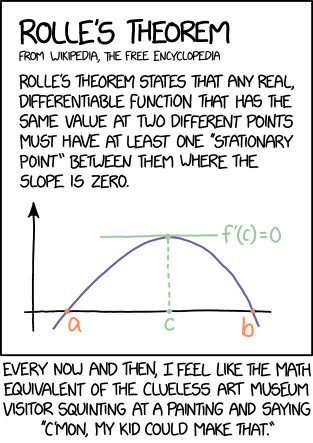
\includegraphics[scale=0.66]{media/xkcd-rolles.png}
	\\ \scriptsize Image from \cite{img:xkcd_rolles}
\end{center}

One can adapt the theorem as follows.
\begin{theorem}
	[Mean value theorem]
	Suppose $f \colon [a,b] \to \RR$ is a continuous function,
	which is differentiable on the open interval $(a,b)$.
	Then there is a point $c \in (a,b)$ such that
	\[ f'(c) = \frac{f(b)-f(a)}{b-a}. \]
\end{theorem}

Pictorially, there is a $c$ such that the tangent at $c$
has the same slope as the secant joining $(a, f(a))$, to $(b, f(b))$;
and Rolle's theorem is the special case where that secant is horizontal.

\begin{center}
\begin{asy}
	import graph;
	size(7cm);
	real f(real x) { return x*x/2 - 0.2; }
	graph.xaxis("$x$");
	graph.yaxis("$y$");
	draw(graph(f,-2,2.5,operator ..), blue, Arrows);
	pair A = (-1, f(-1));
	pair B = (2, f(2));
	dot("$(a, f(a))$", A, dir(A-B), deepgreen);
	dot("$(b, f(b))$", B, dir(10), deepgreen);
	draw(A--B, deepgreen);
	label("Slope $\frac{f(b)-f(a)}{b-a}$", A--B, dir(120), deepgreen);
	draw(A--(A.x,0), deepgreen+dashed);
	draw(B--(B.x,0), deepgreen+dashed);
	label("$a$", (A.x,0), dir(-90), deepgreen);
	label("$b$", (B.x,0), dir(-90), deepgreen);

	real c = (A.y-B.y) / (A.x-B.x);
	pair C = (c, f(c));
	dot("$(c, f(c))$", C, dir(-70), red);
	draw( (c-1, f(c)-c)--(c+1, f(c)+c), red );
\end{asy}
\end{center}

\begin{proof}
	[Proof of mean value theorem]
	Let $s = \frac{f(b)-f(a)}{b-a}$ be the slope of the secant line,
	and define
	\[ g(x) = f(x) - s x \]
	which intuitively shears $f$ downwards so that the
	secant becomes vertical.
	In fact $g(a) = g(b)$ now, so we apply Rolle's theorem to $g$.
\end{proof}

\begin{remark}
	[For people with driver's licenses]
	There is a nice real-life interpretation of this I should mention.
	A car is travelling along a one-dimensional road
	(with $f(t)$ denoting the position at time $t$).
	Suppose you cover $900$ kilometers in your car
	over the course of $5$ hours
	(say $f(0) = 0$, $f(5) = 900$).
	Then there is \emph{some} point at time in which
	your speed at that moment was exactly $180$ kilometers per hour,
	and so you cannot really complain
	when the cops pull you over for speeding.
\end{remark}

The mean value theorem is important because it lets
you relate \textbf{use derivative information
to get information about the function}
in a way that is really not possible without it.
Here is one quick application to illustrate my point:

\begin{proposition}
	[Racetrack principle]
	Let $f, g \colon \RR \to \RR$ be two differentiable functions
	with $f(0) = g(0)$.
	\begin{enumerate}[(a)]
		\ii If $f'(x) \ge g'(x)$ for every $x > 0$,
		then $f(x) \ge g(x)$ for every $x > 0$.
		\ii If $f'(x) > g'(x)$ for every $x > 0$,
		then $f(x) > g(x)$ for every $x > 0$.
	\end{enumerate}
\end{proposition}

This proposition might seem obvious.
You can think of it as a race track for a reason:
if $f$ and $g$ denote the positions of two cars (or horses etc)
and the first car is always faster than the second car,
then the first car should end up ahead of the second car.
At a special case $g = 0$, this says that if $f'(x) \ge 0$,
i.e.\ ``$f$ is increasing'',
then, well, $f(x) \ge f(0)$ for $x > 0$, which had better be true.
However, if you try to prove this by definition from derivatives,
you will find that it is not easy!
However, it's almost a prototype for the mean value theorem.

\begin{proof}
	[Proof of racetrack principle]
	We prove (a). Let $h = f-g$, so $h(0) = 0$.
	Assume for contradiction $h(p) < 0$ for some $p > 0$.
	Then the secant joining $(0, h(0))$ to $(p, h(p))$ has negative slope;
	in other words by mean value theorem there is a $0 < c < p$
	such that
	\[ f'(c) - g'(c) = h'(c) = \frac{h(p)-h(0)}{p} = \frac{h(p)}{p} < 0 \]
	so $f'(c) < g'(c)$, contradiction.
	Part (b) is the same.
\end{proof}

Sometimes you will be faced with two functions which you cannot
easily decouple; the following form may be more useful in that case.
\begin{theorem}
	[Ratio mean value theorem]
	Let $f, g \colon [a,b] \to \RR$ be two continuous functions
	which are differentiable on $(a,b)$,
	and such that $g(a) \neq g(b)$.
	Then there is a $c \in (a,b)$ such that $g'(c) \neq 0$ and
	\[ \frac{f'(c)}{g'(c)} = \frac{f(b)-f(a)}{g(b)-g(a)}. \]
\end{theorem}
\begin{proof}
	Use Rolle's theorem on the function
	\[ h(x) = \left[ f(x)-f(a) \right] \left[ g(b)-g(a) \right]
		- \left[ g(x)-g(a) \right] \left[ f(b)-f(a) \right].
		\qedhere \]
\end{proof}
\begin{remark}
	You can capture the case $g(a) = g(b)$ as well
	if you are willing to write the conclusion
	in the less intuitive form $g'(c) \left[ f(b)-f(a) \right]
	= f'(c) \left[ g(b)-g(a) \right]$.
	In the event $g(a) = g(b)$ then this is just the mean value theorem
	for $g$, and the data of $f$ is irrelevant.
\end{remark}


\section{Smooth functions}
\prototype{All the functions you're used to.}

Let $f \colon U \to \RR$ be differentiable,
thus giving us a function $f' \colon U \to \RR$.
If our initial function was nice enough,
then we can take the derivative again,
giving a function $f'' \colon U \to \RR$, and so on.
In general, after taking the derivative $n$ times,
we denote the resulting function by $f^{(n)}$.
By convention, $f^{(0)} = f$.
\begin{definition}
	A function $f \colon U \to \RR$ is \vocab{smooth}
	if it is infinitely differentiable;
	that is the function $f^{(n)}$ exists for all $n$.
\end{definition}
\begin{ques}
	Show that the absolute value function is not smooth.
\end{ques}

Most of the functions we encounter,
such as polynomials, $e^x$, $\log$, $\sin$, $\cos$
are smooth, and so are their compositions.
Here is a weird example which we'll grow more next time.
\begin{example}
	[A smooth function with all derivatives zero]
	Consider the function
	\[ f(x) = \begin{cases}
			e^{-1/x} & x > 0 \\
			0 & x \le 0.
		\end{cases}
	\]
	This function can be shown to be smooth,
	with $f^{(n)}(0) = 0$.
	So this function has every derivative at the origin
	equal to zero, despite being nonconstant!
\end{example}

\section{\problemhead}
\begin{problem}
	[Quotient rule]
	Let $f \colon (a,b) \to \RR$ and $g \colon (a,b) \to \RR_{>0}$
	be differentiable functions.
	Let $h = f/g$ be their quotient
	(also a function $(a,b) \to \RR$).
	Show that the derivative of $h$ is given by
	\[ h'(x) = \frac{f'(x) g(x) - f(x) g'(x)}{g(x)^2}. \]
\end{problem}

\begin{problem}
	For real numbers $x > 0$, how small can $x^x$ be?
\end{problem}

\begin{problem}
	[RMM 2018]
	\gim
	Determine whether or not there exist
	nonconstant polynomials $P(x)$ and $Q(x)$ with
	real coefficients satisfying
	\[ P(x)^{10} + P(x)^9 = Q(x)^{21} + Q(x)^{20}. \]
\end{problem}

\begin{problem}
	\gim
	Let $P(x)$ be a degree $n$ polynomial with real coefficients.
	Prove that the equation $e^x = P(x)$ has at most $n+1$ real solutions in $x$.
\end{problem}

\begin{problem}
	[Jensen's inequality]
	Let $f \colon (a,b) \to \RR$ be a twice differentiable function
	such that $f''(x) \ge 0$ for all $x$
	(i.e.\ $f$ is \emph{convex}).
	Prove that
	\[ f\left( \frac{x+y}{2} \right)
		\le \frac{f(x) + f(y)}{2} \]
	for all real numbers $x$ and $y$ in the interval $(a,b)$.
\end{problem}

\begin{problem}
	[L'H\^{o}pital rule, or at least one case]
	Let $f,g \colon \RR \to \RR$ be differentiable functions
	and let $p$ be a real number.
	Suppose that
	\[ \lim_{x \to p} f(x) = \lim_{x \to p} g(x) = 0. \]
	Prove that
	\[ \lim_{x \to p} \frac{f(x)}{g(x)}
		= \lim_{x \to p} \frac{f'(x)}{g'(x)} \]
	provided the right-hand limit exists.
\end{problem}

